\subsection{Построения циркулем и линейкой}

\begin{definition}
	Заданы точки $0, 1 \in \Cm$. При \textit{построениях циркулем и линейкой} разрешается производить следующие операции:
	\begin{enumerate}
		\item Провести прямую через две уже построенные точки
		\item Провести окружность с центром в уже построенной точке и радиусом, равном расстоянию между двумя уже построенными точками
		\item Построить точку на пересечении проведенных прямых и окружностей
	\end{enumerate}

	Будем говорить, что точку $z \in \Cm$ \textit{можно построить циркулем и линейкой}, если существует конечная последовательность операций, в ходе которой будет построена $z$.
\end{definition}

\begin{proposition}
	Если можно построить точки $z, w \in \Cm$, то можно построить $z + w$, точки $\lambda z$ для любого $\lambda \in \Q$, $z \cdot w$, $\frac 1z$ при $z \ne 0$, $\sqrt{z}$.
\end{proposition}

\begin{proof}
	Заметим сначала, что с помощью циркуля и линейки можно строить прямые, параллельные, а также откладывать расстояния, равные заданному. Тогда точки $\lambda z$ и $z + w$ можно построить следующим образом:
	\begin{center}
		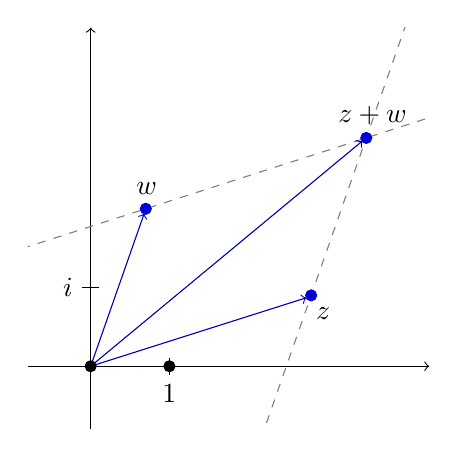
\begin{tikzpicture}
			\clip (-0.8, -0.8) rectangle (4.3, 4.3);
			\draw [->] (-0.8, 0) -- (4.3, 0);
			\draw [->] (0, -0.8) -- (0, 4.3);
			
			\draw (1,3pt) -- (1,-3pt) node [below, black] {$1$};
			\draw (3pt,1) -- (-3pt,1) node [left, black] {$i$};
			
			% прямые пунктиром
			\draw [style=help lines,dashed, thin, gray] (0.7-3 * 2.8, 2-3 * 0.9) -- (0.7 + 3 * 2.8, 2 + 3 * 0.9);
			\draw [style=help lines,dashed, thin, gray] (2.8 -3 * 0.7, 0.9-3 * 2) -- (2.8 + 3 * 0.7, 0.9 + 3 * 2);
			
			\draw [->, black!30!blue] (0, 0) -- (2.74, 0.87) node [black, below right] {$z$};
			\draw [->, black!30!blue] (0, 0) -- (0.68, 1.94) node [black, xshift=0.03cm, yshift=0.32cm] {$w$};
			\draw [->, black!30!blue] (0, 0) -- (3.45, 2.86) node [black, yshift=0.32cm, xshift=0.13cm] {$z + w$};
			
			\node[draw,circle,inner sep=1.4pt,fill] at (0, 0) {};
			\node[draw,circle,inner sep=1.4pt,fill] at (1, 0) {};
			
			\node[draw,circle,inner sep=1.4pt,fill,black!15!blue] at (2.8, 0.9) {};
			\node[draw,circle,inner sep=1.4pt,fill,black!15!blue] at (0.7, 2) {};
			\node[draw,circle,inner sep=1.4pt,fill,black!15!blue] at (2.8 + 0.7, 0.9 + 2) {};
		\end{tikzpicture}\quad\quad
		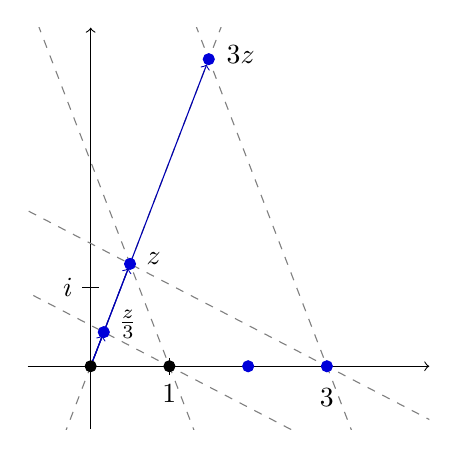
\begin{tikzpicture}
			\clip (-0.8, -0.8) rectangle (4.3, 4.3);
			\draw [->] (-0.8, 0) -- (4.3, 0);
			\draw [->] (0, -0.8) -- (0, 4.3);
			
			\draw (1,3pt) -- (1,-3pt) node [below, black] {$1$};
			\draw (3pt,1) -- (-3pt,1) node [left, black] {$i$};
			\draw (3,1pt) -- (3,-1pt) node [yshift=-0.362cm, black] {$3$};
			
			\draw [style=help lines,dashed, thin, gray] (-9 * 0.5, -9 * 1.3) -- (9 * 0.5, 9 * 1.3);
			\draw [style=help lines,dashed, thin, gray] (1 + 9 * 0.5, -9 * 1.3) -- (1 - 9 * 0.5, 9 * 1.3);
			\draw [style=help lines,dashed, thin, gray] (3 + 9 * 0.5, -9 * 1.3) -- (3 - 9 * 0.5, 9 * 1.3);
			\draw [style=help lines,dashed, thin, gray] (3 + 9 * 2.5, -9 * 1.3) -- (3 - 9 * 2.5, 9 * 1.3);
			\draw [style=help lines,dashed, thin, gray] (1 + 9 * 2.5, -9 * 1.3) -- (1 - 9 * 2.5, 9 * 1.3);
			
			\draw [->, black!30!blue] (0, 0) -- (0.5 * 0.96, 1.3 * 0.96) node [black, xshift=0.32cm, yshift=0.12cm] {$z$};
			\draw [->, black!30!blue] (0, 0) -- (0.5 * 2.95, 1.3 * 2.95) node [black, xshift=0.43cm, yshift=0.12cm] {$3z$};
			\draw [->, black!30!blue] (0, 0) -- (0.5 / 3.3, 1.3 / 3.3) node [black, xshift=0.32cm, yshift=0.14cm] {$\frac{z}{3}$};
			
			\node[draw,circle,inner sep=1.4pt,fill,black!15!blue] at (0.5, 1.3) {};
			\node[draw,circle,inner sep=1.4pt,fill,black!15!blue] at (0.5 / 3, 1.3 / 3) {};
			\node[draw,circle,inner sep=1.4pt,fill,black!15!blue] at (0.5 * 3, 1.3 * 3) {};
			
			\node[draw,circle,inner sep=1.4pt,fill] at (0, 0) {};
			\node[draw,circle,inner sep=1.4pt,fill] at (1, 0) {};
			\node[draw,circle,inner sep=1.4pt,fill, black!15!blue] at (2, 0) {};
			\node[draw,circle,inner sep=1.4pt,fill, black!15!blue] at (3, 0) {};
		\end{tikzpicture}
	\end{center}
	
	Построение точек $|w|z$ и $\frac{1}{z}$ аналогично построению точки $\lambda z$. Кроме того, поскольку с помощью циркуля и линейки можно откладывать угол, равный заданному, то построить можно и $z \cdot w$. Покажем теперь, как построить $\sqrt{|z|}$:
	\begin{center}
	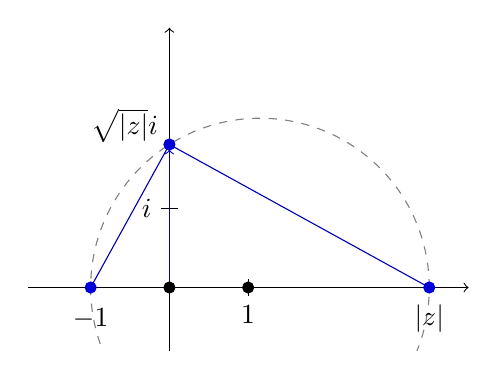
\begin{tikzpicture}
		\clip (-1.8, -0.8) rectangle (3.8, 3.3);
		\draw [->] (-1.8, 0) -- (3.8, 0);
		\draw [->] (0, -0.8) -- (0, 3.3);
		
		\draw (1,3pt) -- (1,-3pt) node [below, black] {$1$};
		\draw (3pt,1) -- (-3pt,1) node [left, black] {$i$};
		
		\draw [->, black!30!blue] (0, 0) -- (0, 1.81659 - 0.064) node [black, xshift = -0.57cm, yshift=0.3cm] {$\sqrt{|z|}i$};
		\draw [black!30!blue] (-1, 0) -- (0, 1.81659) node [black, below right] {};
		\draw [black!30!blue] (3.3, 0) -- (0, 1.81659) node [black, below right] {};
		\draw[style=help lines,dashed, thin, gray] (2.3 / 2, 0) circle[radius=2.3 / 2 + 1];
		
		\draw (3.3,1pt) -- (3.3,-1pt) node [yshift=-0.362cm, black] {$|z|$};
		\draw (-1,1pt) -- (-1,-1pt) node [yshift=-0.362cm, black] {$-1$};
		
		\node[draw,circle,inner sep=1.4pt,fill] at (0, 0) {};
		\node[draw,circle,inner sep=1.4pt,fill] at (1, 0) {};
		\node[draw,circle,inner sep=1.4pt,fill, black!15!blue] at (-1, 0) {};
		\node[draw,circle,inner sep=1.4pt,fill, black!15!blue] at (3.3, 0) {};
		\node[draw,circle,inner sep=1.4pt,fill, black!15!blue] at (0, 1.81659) {};
	\end{tikzpicture}
	\end{center}

	Наконец, с помощью циркуля и линейки можно делить заданный угол пополам, поэтому построить можно и $\sqrt{z}$.
\end{proof}

\begin{corollary}
	Если можно построить точки $z, w \in \Cm$, то можно построить любую точку из поля $\Q(z, w)$.
\end{corollary}

\begin{theorem}
	Точку $z \in \Cm$ можно построить циркулем и линейкой $\lra$ существует башня расширений $K_0 \supset \dotsb \supset K_n = \Q$ такая, что $z \in K_0$ и для каждого $i \in \{0, \dotsc, n - 1\}$ выполнено $[K_i : K_{i + 1}] = 2$.
\end{theorem}

\begin{proof}~
	\begin{itemize}
		\item[$\la$] Заметим, что расширение степени $2$ "--- это расширение, полученное добавлением корня квадратного уравнения, поскольку если $\alpha \in K_i \backslash K_{i + 1}$, то система $(1, \alpha, \alpha^2)$ линейно зависима. Тогда, по индукции, все точки каждого из расширений можно построить.
		\item[$\ra$] Пусть точку $z \in \Cm$ можно построить. Рассмотрим набор последовательно построенных точек $0, 1, z_1, \dotsc, z_n = z$. Заметим, что $x + yi \in \Cm$ можно построить тогда и только тогда, когда $x, y \in \R$ можно построить, и перейдем к рассмотрению набора $0, 1, i, x_1 := \re{z_1}, y_1 := \im{z_1}, \dotsc, x_n, y_n$. Достаточно по индукции показать, что для всех $i \in \{0, \dotsc, n - 1\}$ выполнено $[\Q(i, x_1, y_1, \dotsc, x_{i + 1}, y_{i + 1}) : \Q(i, x_1, y_1, \dotsc, x_{i}, y_{i})] \le 2$.
		
		Рассмотрим для примера только случай, когда очередная точка $w$ получена как пересечение прямой, проходящей через точки $w_1, w_2$, и окружности с центром $w_3$, проходящей через точку $w_4$.
		\begin{center}
			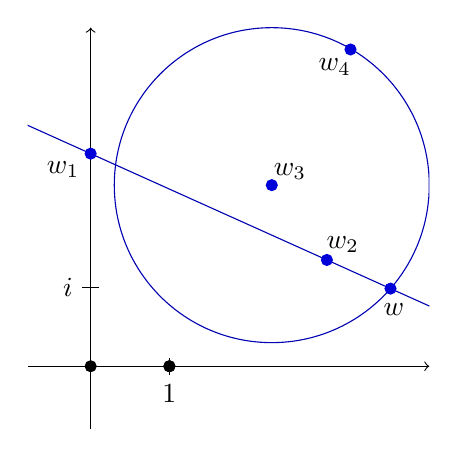
\begin{tikzpicture}
				\clip (-0.8, -0.8) rectangle (4.3, 4.3);
				\draw [->] (-0.8, 0) -- (4.3, 0);
				\draw [->] (0, -0.8) -- (0, 4.3);
				
				\draw (1,3pt) -- (1,-3pt) node [below, black] {$1$};
				\draw (3pt,1) -- (-3pt,1) node [left, black] {$i$};
				
				\draw[black!30!blue] (2.3, 2.3) circle[radius=2];
				\node[draw,circle,inner sep=1.4pt,fill] at (1, 0) {};
				\draw [black!30!blue] (0 - 3, 2.7 + 1.35) -- (3 + 3, 1.35 - 1.35);
				
				\node[draw,circle,inner sep=1.4pt,fill, black!15!blue] at (0, 2.7) {};
				\node[black] at (-0.35, 2.5) {$w_1$};
				\node[draw,circle,inner sep=1.4pt,fill, black!15!blue] at (3, 1.35) {};
				\node[black] at (3.2, 1.55) {$w_2$};
				\node[draw,circle,inner sep=1.4pt,fill, black!15!blue] at (2.3, 2.3) {};
				\node[black] at (2.53, 2.47) {$w_3$};
				\node[draw,circle,inner sep=1.4pt,fill, black!15!blue] at (3.3, 4.023) {};
				\node[black] at (3.1, 3.8) {$w_4$};
				\node[draw,circle,inner sep=1.4pt,fill, black!15!blue] at (3.808, 0.986) {};
				\node[black] at (3.85, 0.72) {$w$};
				
				\node[draw,circle,inner sep=1.4pt,fill] at (0, 0) {};
				\node[draw,circle,inner sep=1.4pt,fill] at (1, 0) {};
			\end{tikzpicture}
		\end{center}
		
		 Обозначим координаты точек $w_1, \dotsc, w_4, w$ через $(x_1, y_1), \dotsc, (x_4, y_4), (x, y)$. Тогда точка $w$ является решением следующей системы уравнений:
		\[\left\{\begin{aligned}
			&(x - x_1)(y - y_2) = (x - x_2)(y - y_1)\\
			&(x - x_3)^2 + (y - y_3^2) = (x_4 - x_3)^2 + (y_4 - y_3^2)
		\end{aligned}\right.\]
		
		Из этой системы видно, что $x, y$ линейно зависимы над $\Q(x_1, x_2, y_1, y_2)$ и $x$ является решением квадратного уравнения с коэффициентами из $\Q(x_1, y_1 \dotsc, x_4, y_4)$, поэтому $[\Q(i, x_1, y_1 \dotsc, x_4, y_4, x, y) : \Q(i, x_1, y_1 \dotsc, x_4, y_4)] \le 2$.\qedhere
	\end{itemize}
\end{proof}

\begin{corollary}
	Если точку $z \in \Cm$ можно построить, то $z \in K$ для некоторого расширения $K \supset \Q$ такого, что $[K : \Q] = 2^n$, $n \in \N$.
\end{corollary}

\begin{corollary}
	Если минимальный многочлен $m_z$ числа $z \in \Cm$ имеет степень $\deg{m_z} \ne 2^n$, $n \in \N$, то $z$ нельзя построить.
\end{corollary}

\begin{proof}
	Любое расширение $L \supset \Q$, содержащее $z$, является также расширением поля $\Q(z)$ и потому имеет степень, кратную $\deg{m_z}$, то есть отличную от степени двойки. Значит, $z$ нельзя построить.
\end{proof}

\begin{theorem}
	Следующие задачи нельзя решить с помощью циркуля и линейки:
	\begin{itemize}
		\item Удвоение куба (построение куба, имеющего вдвое больший объем, чем заданный куб)
		\item Трисекция угла (разбиение заданного угла на три равные части)
		\item Квадратура круга (построение квадрата, имеющего площадь заданного круга)
	\end{itemize}
\end{theorem}

\begin{proof}
	Достаточно заметить, что задачи выше эквивалентны построению чисел $\sqrt{3}$, $\sin\frac{\pi}{18}$ (при условии, что задан угол $\frac{\pi}{6}$) и $\sqrt\pi$ соответственно. Ни одно из этих чисел нельзя построить.
\end{proof}

\begin{note}
	Построение правильного $n$-угольника с помощью циркуля и линейки эквивалентно построению числа $\xi_n = e^{\frac{2\pi i}{n}}$. Далее в курсе мы докажем, что число $\xi_n$ можно построить $\lra$ $\phi(n) = 2^k$, $k \in \N$.
\end{note}